\chapter{Mention2Vec Models}

In this chapter, we introduce multitask models based on Mention2Vec. We conduct experiments using the multitask models on sequence tagging tasks and compare their performance and decoding speed with Feedforward and BiLSTM-CRF

\section{Model Description}

\subsection{Feedforward-Mention2Vec for NER}

Mention2Vec is a neural network model for NER, which uses BiLSTMs to predict boundaries and entity types separately (\citeauthor{stratos2016mention2vec}, \citeyear{stratos2016mention2vec}). We summarize Mention2Vec into two steps. The first step uses a BiLSTM to generate hidden embeddings the same way in the BiLSTM-CRF model and predicts the boundaries using hidden embeddings. Unlike usual NER labels (B-LOC, I-LOC, \dots), boundary labels in this step do not have NER types attached. Since the boundary labels have strong correlations, Mention2Vec uses CRF to capture correlations and produce boundary label sequences.

Figure \ref{fig:mention2vec1} illustrates the first step of Mention2Vec on an NER example. We denote the input word sequence as $W: \left\{w_{1}, w_{2}, \dots, w_{n}\right\}$, input embeddings as $X: \left\{x_{1}, x_{2}, \dots, x_{n}\right\}$ which are the concatenations of the character embeddings and the word embeddings, and the hidden embeddings as $H: \left\{h_{1}, h_{2}, \dots, h_{n}\right\}$. 

\begin{figure}
  \centering
  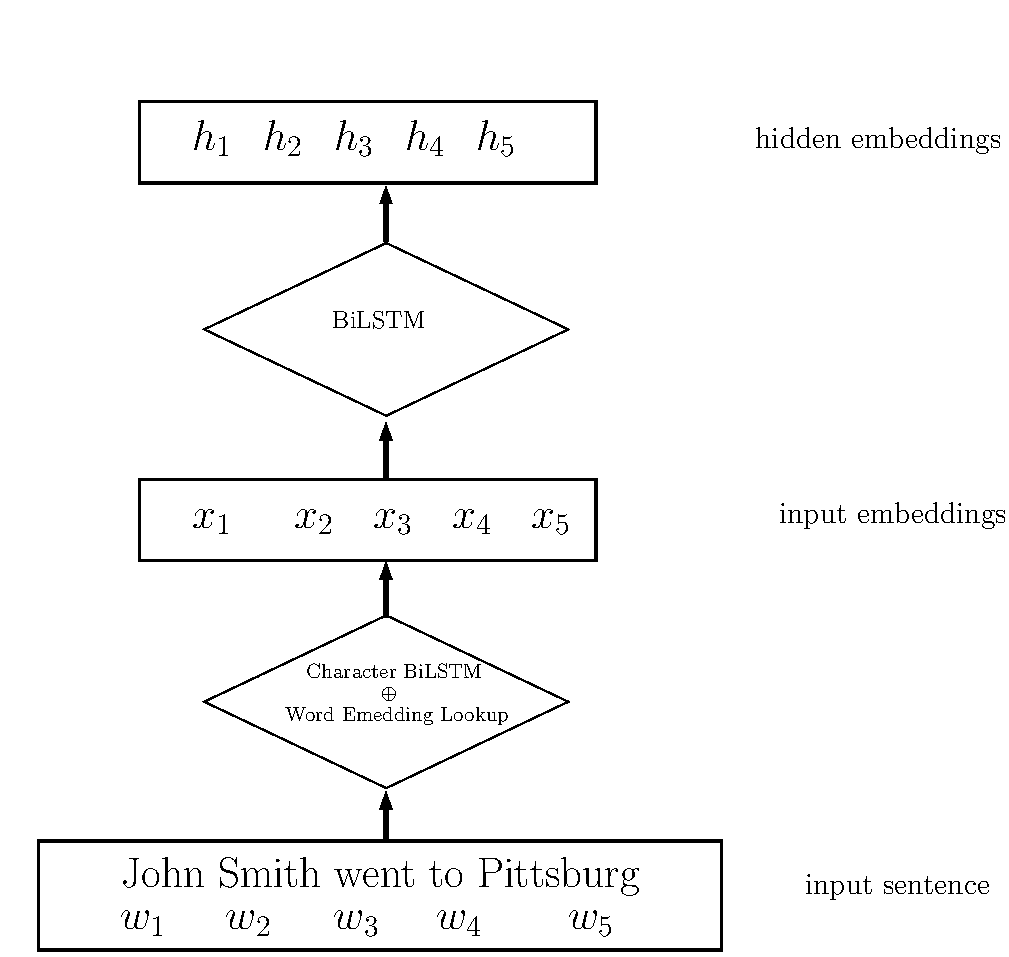
\includegraphics[scale=0.6]{mention2vec1.pdf}
 \caption{The first step of Mention2Vec for NER}
  \label{fig:mention2vec1}
\end{figure}

The output boundary label probability distribution is denoted as $p_{i}$ for word $w_{i}$, and the gold boundary label sequence is denoted as $Y_{label}$. In each training step, the boundary detection loss is given by the negative log likelihood of the gold boundary label sequence, shown in Equation \ref{eqn:loss1}

\begin{equation}\label{eqn:loss1}
  L_{1}\left(\theta _{1}\right) =-\log \left( p\left( Y_{label}|h_{1}, h_{2} \dots h_{n}\right) \right) 
\end{equation}

\begin{figure}
  \centering
  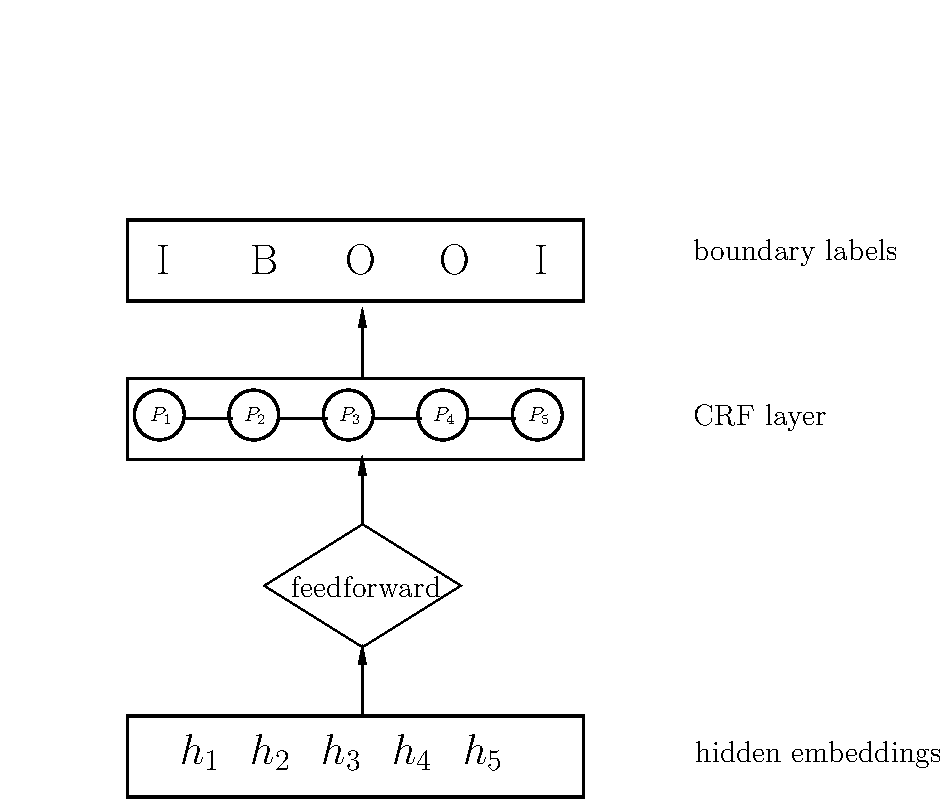
\includegraphics[scale=0.6]{mention2vec2.pdf}
 \caption{The second step of Mention2Vec for NER}
  \label{fig:mention2vec2}
\end{figure}

The second step of Mention2Vec is type prediction which finds actual types for named entity spans in a sequence. It makes use of the hidden embeddings and the entity boundaries from the first step. The model first looks up the hidden embeddings for the words in entity spans. Then, it feeds the hidden embeddings into an additional BiLSTM and obtains the type probability distributions. Figure \ref{fig:mention2vec2} illustrates the third step of Mention2Vec.

The gold type output of an input sequence is denoted as $Y_{type}$. Assuming there are $l$ named entities in a sequence, and the index of the first word in a named entity is represented as $s$, and the index of the last word in a named entity is represented as $e$, the type prediction loss is computed by \ref{eqn:loss2}:

\begin{equation}\label{eqn:loss2}
  L_{2}\left(\theta _{2}\right) =-\sum _{l}\log P\left( r^{l}|h_{s}^{l}{\ldots }h_{e}^{l}\right)
\end{equation}

During training, the model uses the gold boundaries and gold types to compute the boundary detection loss and the type prediction loss. In each training step, the boundary detection loss and the type prediction loss are minimized jointly: the training objective is to find boundary sequences and type sequences that minimize the sum of $L_{1}$ and $L_{2}$.


In order to further speed up Mention2Vec as well as capture the correlation between boundary tags, we consider using a different network for boundary detection. Shown in Chapter 3, feedforward networks can produce relatively good performance on sequence tagging with faster speed than BiLSTM. We then replace the BiLSTM in the first step of Mention2Vec with a feedforward network. We denote this new model as Feedforward-Mention2Vec. Feedforward-Mention2Vec still has two steps where the second step is the same in Mention2Vec. The first step uses a feedforward network to produce the hidden embeddings, which is illustrated in Figure \ref{fig:mention2vec3}.

\begin{figure}
  \centering
  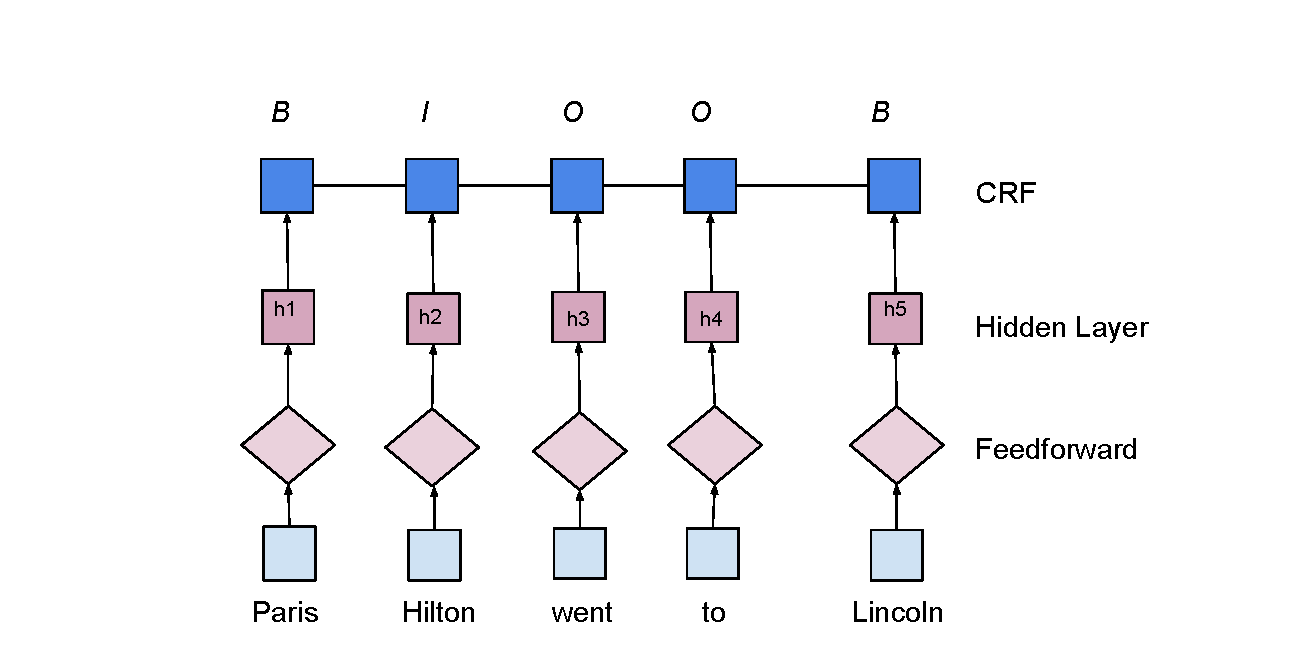
\includegraphics[scale=0.6]{mention2vec3.pdf}
 \caption{The first step of Feedforward-Mention2Vec}
  \label{fig:mention2vec3}
\end{figure}

In both Feedforward-Mention2Vec and Mention2Vec, the run time of decoding boundaries is constant with the number of types, since there are only three types of boundaries (I, O, B) to decode in the CRF layer. In other CRF based models, like BiLSTM-CRF, the decoding time grows quadratically in the number of named entity types. 

\subsection{BPE-Mention2Vec for POS}
In POS, each word in the input sentence is assigned a unique part-of-speech tag. Since there is no tag span existing in POS, it's not necessary to use a multitask model on POS. However, we propose a way to convert POS into an NER-like task through the help of Byte Pair Encoding. Inspired by the successful results obtained by using BPE in machine translation (\citeauthor{sennrich2015neural}, \citeyear{sennrich2015neural}), we initially wanted to use BPE to capture morphological decomposition of the words and replace spelling features like prefixes and suffixes. BPE is a compression algorithm which replaces frequent pairs with an unused byte. \cite{sennrich2015neural} presents a way to adapt BPE for word segmentation: using BPE to segment words into subword units of different length, and building a vocabulary dictionary using word frequency. In POS tagging system, we first learn BPE merge operations on the training data. To segment training data and test data, we first split each word in characters and then apply BPE to merge characters into larger chunks. In order to restore the words, we use the ``IOB'' label scheme to label the subword units. Since there can be multiple subword units sharing the same tag, POS becomes a task similar with NER. Figure \ref{fig:bpe} shows an example of using BPE to segment a sequence with POS tags. 

\begin{figure}[h]
  \centering
  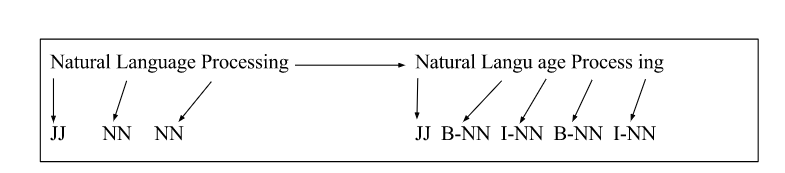
\includegraphics[scale=0.5]{bpe.png}
 \caption{An example of using BPE for word segmentation}
  \label{fig:bpe}
\end{figure}

In our proposed BPE-Mention2Vec model for POS, there are three main steps. In the first step, given a sequence, we use BPE to segment the words and convert the corresponding tags using the ``IOB'' label scheme. After the first step, we have an NER-like task with known boundary of each entity span, so we can apply the same method in Feedforward-Mention2Vec to predict the POS types for entity spans. In the second step, we use a feedforward network to produce the hidden embeddings of the input words. CRF is not used here because the boundary labels are known in both training and decoding. The third step of BPE-Mention2Vec uses a BiLSTM to predict the POS tags for each entity span based on the hidden embeddings and the known boundaries. Figure \ref{fig:bpemention2vec} describes the process of using BPE-Mention2Vec to find POS tags for a sequence. 

\begin{figure}
  \centering
  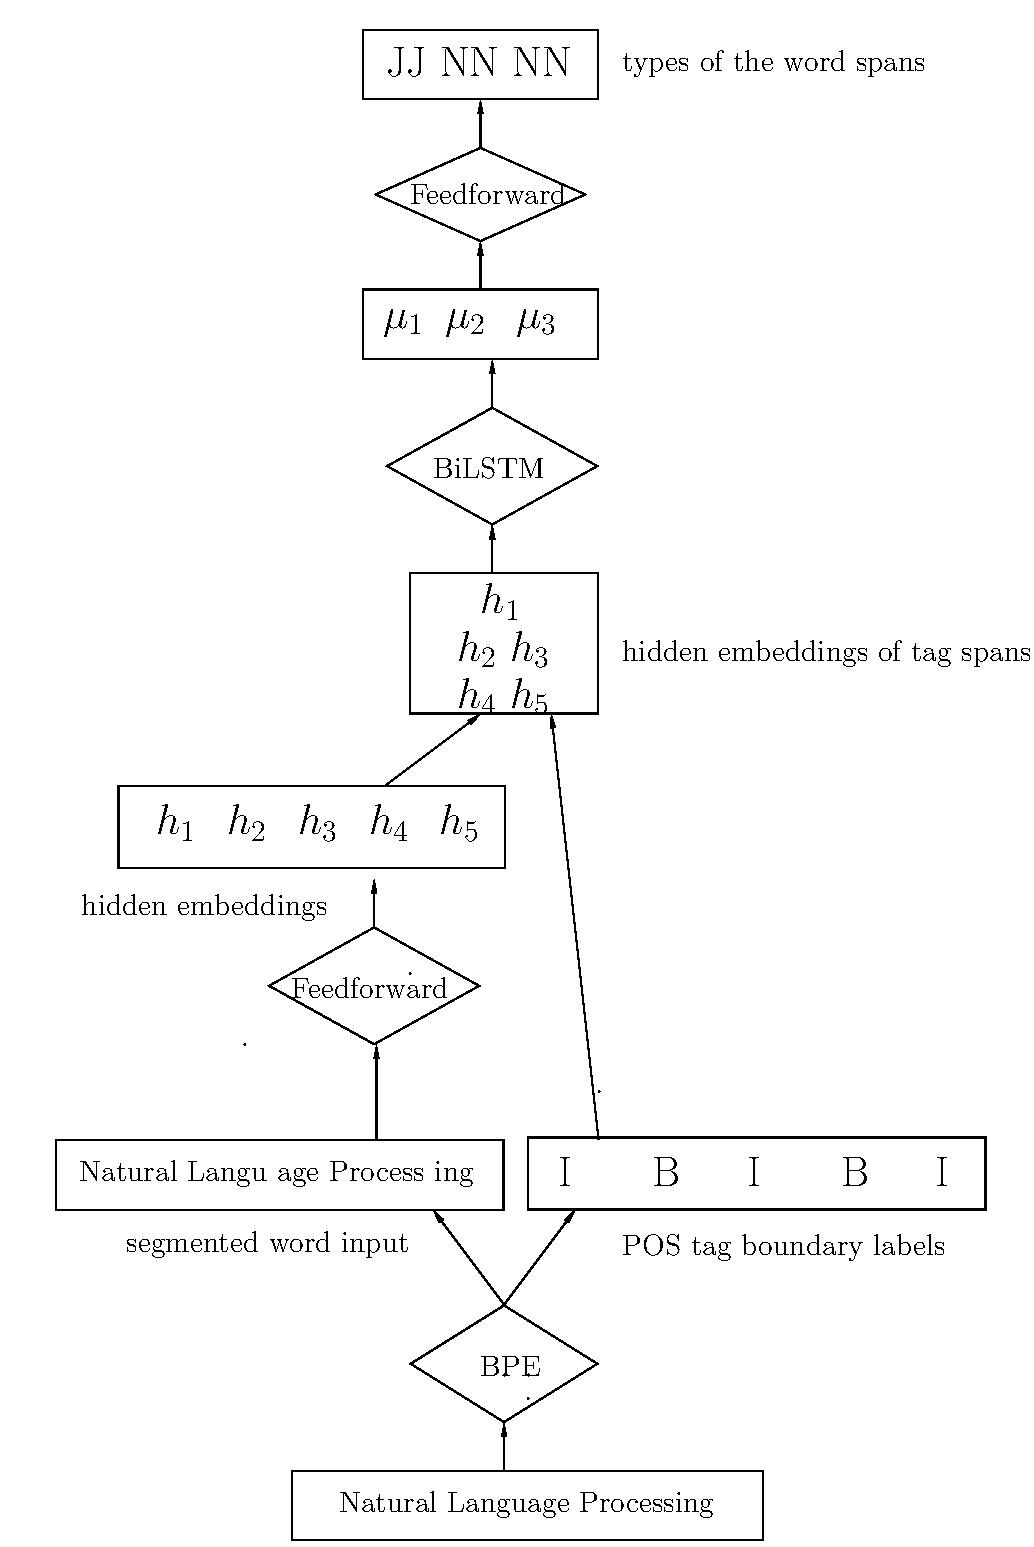
\includegraphics[scale=0.6]{bpemention2vec.pdf}
 \caption{An example of using BPE-Mention2Vec to find POS tags}
  \label{fig:bpemention2vec}
\end{figure}

\section{Experiments and Results}

We empirically evaluate the Mention2Vec model and the Feedforward-Mention2Vec model for NER, and the BPE-Mention2Vec model for POS. The hardware specifications are listed in Table \ref{table:hardware}. The experiments were conducted on a Linux server with a single 10G Nvidia GeForce GPU. The experiments specification is shown in Table \ref{table:hardware}. In the implementation of Mention2Vec, we use the same set of hyperparameters from the origin model (\citeauthor{stratos2016mention2vec}, \citeyear{stratos2016mention2vec}). We perform minimum hyperparameter tuning for Feedforward-Mention2Vec and BPE-Mention2Vec over hidden layer size, learning rate, and dropout rate. The hyperparameters we use in Feedforward-Mention2Vec and BPE-Mention2Vec are shown in Table \ref{table:hyperparameters3}.

\begin{table}[h]
\centering
\caption{Hyperparameters used in Feedforward-Mention2Vec and BPE-Mention2Vec}
\label{table:hyperparameters3}
\begin{tabular}{|c|c|}
\hline
Hyperparameters & Values \\ \hline
character embedding size & 50 \\ \hline
word embedding size & 100 \\ \hline
feedforward layer size & 200 \\ \hline
feedforward layer & 1 \\ \hline
optimizer & Adam \\ \hline
learning rate & 0.001 \\ \hline
batch size & 32 \\ \hline
dropout rate & 0.5 \\ \hline
\end{tabular}
\end{table}

\begin{table}[h]
\centering
\caption{NER F1 Score and Decoding Speed Comparison on CoNLL 2003}
\label{table:ner-mention2vec1}
\begin{tabular}{|c|c|c|c|c|}
\hline
Model   & Precision & Recall & F1 & Speed \\ \hline
Feedforward &82.99 &83.59 &83.29 & 26819 \\ \hline
BiLSTM-CRF &89.93 &90.16 &\textbf{90.05} (+6.76) & 10100 (-2.65$\times$) \\ \hline
Mention2Vec &89.14 &88.99 &89.06 (+5.77) & 9701 (-2.76$\times$) \\ \hline
Feedforward-Mention2Vec &88.98 &88.21 &88.6 (+5.31) & 13450 (-1.99$\times$) \\ \hline
\end{tabular}
\bigskip
\caption{Chunking F1 Score and Decoding Speed Comparison on CoNLL 2000}
\label{table:chunk-mention2vec1}
\begin{tabular}{|c|c|c|c|c|}
\hline
Model   & Precision & Recall & F1 & Speed \\ \hline
Feedforward & 89.35 &91.55 &90.43 & 16920 \\ \hline
BiLSTM-CRF &93.91 &93.81 &\textbf{93.86} (+3.43) & 5390 (-3.14$\times$) \\ \hline
Mention2Vec &93.03 & 93.13 &93.08 (+2.65) & 5465 (-3.09$\times$) \\ \hline
Feedforward-Mention2Vec &92.61 & 92.62 &92.61 (+2.18) & 7601 (-2.23$\times$) \\ \hline
\end{tabular}
\end{table}

\begin{table}[h]
\centering
\caption{NER F1 Score and Decoding Speed Comparison on OntoNotes}
\label{table:ner-mention2vec2}
\begin{tabular}{|c|c|c|c|c|}
\hline
Model & Precision & Recall & F1 & Speed(words/sec) \\ \hline
Feedforward  & 82.98 & 62.09 & 71.03 & 22829 \\ \hline
BiLSTM-CRF &86.59 &85.21 &\textbf{85.90} & 7667 (-2.97$\times$)
  \\ \hline
Mention2Vec & 86.24 & 84.25 & 85.23 & 8433 (-2.71$\times$)
         \\ \hline
Feedforward-Mention2Vec & 85.40 & 79.92 & 82.57 & 10812 (-2.11$\times$) \\ \hline
\end{tabular}
\bigskip
\caption{Per-label F1 Score on OntoNotes}
\label{table:ner-mention2vec3}
\begin{tabular}{|c|c|c|c|}
\hline
Labels             & Feedforward & Feedforward-Mention2Vec & BiLSTM-Char-CRF \\ \hline
         CARDINAL  & 72.38  & 78.03  & 80.33 \\ \hline
             DATE: & 72.45  & 80.61  & 81.24 \\ \hline
            EVENT: & 30.01  & 45.81  & 61.40 \\ \hline
              FAC: & 29.08  & 46.27  & 57.94 \\ \hline
              GPE: & 89.62  & 92.84  & 94.84 \\ \hline
         LANGUAGE: & 45.16  & 43.42  & 51.43 \\ \hline
              LAW: & 20.02  & 43.62  & 57.97 \\ \hline
              LOC: & 52.79  & 64.71  & 73.51 \\ \hline
            MONEY: & 77.73  & 81.66  & 86.98 \\ \hline
             NORP: & 84.11  & 87.80  & 92.15 \\ \hline
          ORDINAL: & 71.26  & 72.77  & 77.24 \\ \hline
              ORG: & 72.05  & 79.92  & 85.27 \\ \hline
          PERCENT: & 84.43  & 89.27  & 88.73 \\ \hline
           PERSON: & 82.72  & 86.98  & 90.65 \\ \hline
          PRODUCT: & 51.66  & 50.00  & 64.38 \\ \hline
         QUANTITY: & 65.78  & 74.77  & 81.13 \\ \hline
             TIME: & 41.68  & 56.44  & 58.85 \\ \hline
      WORK OF ART: & 26.29  & 37.63  & 47.21 \\ \hline
\end{tabular}
\end{table}


In Chunking and NER experiments, we compare Feedforward-Mention2Vec with Mention2Vec on the CoNLL 2003 data set. We use the BiLSTM-CRF and Feedforward as baseline models because BiLSTM-CRF achieves the highest F1 score and Feedforward has the fastest decoding speed among the previous models we built. Table \ref{table:ner-mention2vec1} shows the NER performance and decoding speed of these neural network models on the CoNLL 2003 data set.Table \ref{table:chunk-mention2vec1} shows the Chunking performance and decoding speed of these neural network models on the CoNLL 2000 data set. Mention2Vec and Feedforward-Mention2Vec obtain lower F1 score than BiLSTM-CRF. Feedforward-Mention2Vec is faster than Mention2Vec and BiLSTM-CRF. The empirical results demonstrate that the Feedforward-Mention2Vec model performs competitively on Chunking and NER while being faster than original Mention2Vec model and the state-of-the-art model. Feedforward is still the fastest but it has the lowest F1 score on both tasks.

Different NER corpus may have different named entity types. We have noted that Feedforward-Mention2Vec and Mention2Vec scale linearly in the number of named entity types while BiLSTM-CRF grows quadratically. We want to show the time difference of the same model on NER data sets with different numbers of named entity types. We have obtained the performance and decoding speed of these models on CoNLL 2003 which has 4 types of named entity. Then we conduct the experiments on the OntoNotes English data set which has 18 types of named entity. Table \ref{table:ner-mention2vec2} reports the final results of the experiments. The same model obtains lower F1 score on OntoNotes. Table \ref{table:ner-mention2vec3} shows the per label performance of Feedforward-Mention2Vec, BiLSTM-CRF, and Feedforward. They reveal that some labels in OntoNotes are classified poorly, such as ``WORK OF ART'' and ``LANGUAGE''. We suspect this is due to OntoNotes is more noisy than CoNLL 2003 as OntoNotes data is extracted from a wide variety of sources with more named entity types. In terms of decoding speed, while Feedforward-Mention2Vec is 1.3 times faster than the BiLSTM-CRF model on the data set with 4 named entity types, Feedforward-Mention2Vec is 1.4 times faster on the data set with 18 named entity types. Mention2Vec is slightly slower than BiLSTM--CRF on CoNLL 2003, but it's faster than BiLSTM-CRF on OntoNotes.

\begin{table}[h]
\centering
\caption{POS Tagging Systems Performance and speed Comparison}
\label{table:pos-mention2vec}
\begin{tabular}{|c|c|c|c|}
\hline
Model   & Accuracy & Error Reduction & Speed \\ \hline
Feedforward     & 95.89  & $-$ & 30967  \\ \hline
BPE-Mention2Vec & 96.04 (+0.15) &85 & 4923 (-6.29$\times$)   \\ \hline
BILSTM-CRF & 97.34 (+1.45) &822 & 9009 (-3.43$\times$) \\ \hline
\end{tabular}
\end{table}

In the POS experiments, we compare BPE-Mention2Vec with BiLSTM-CRF which is the state-of-the-art model for POS, and with Feedforward which is the fastest among the models we have built. Table \ref{table:pos-mention2vec} demonstrates the performance and decoding speed of them on the Penn Treebank data set. BPE-Mention2Vec obtains lower accuracy than BiLSTM-CRF and higher accuracy than Feedforward. Since using word segmentation increases the number of words to be processed and introduces more preprocessing time, BPE-Mention2Vec is slower than the BiLSTM-CRF and Feedforward. The empirical results conclude that BiLSTM-CRF is a better model than BPE-Mention2Vec on POS. 
